
%%%%%%%%%%%%%%%%%%%%%%%%%%%%%%%%%%%%%%%%%%%%%%%%%%%%%%%%%%%
%%%%%%%%%%%%%%%%%%%%%%%%%%%%%%%%%%%%%%%%%%%%%%%%%%%%%%%%%%%
\subsection{XRD}
\begin{figure}
	\centering
	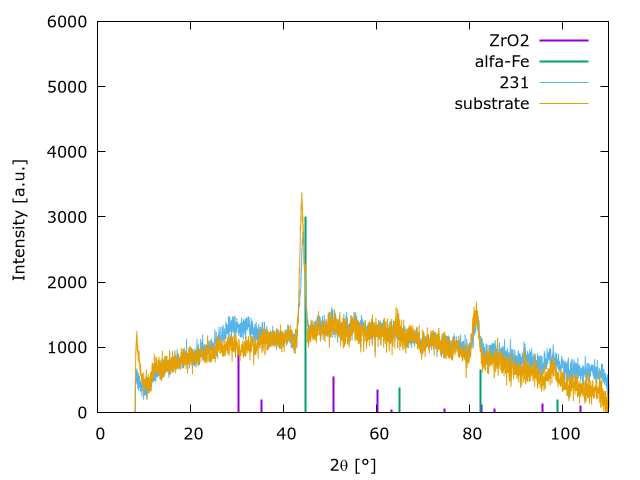
\includegraphics[width=\picwidth]{Pics/xrd.png}
	\caption{XRD spectra}
	\label{fig:xrd}
\end{figure}

%%%%%%%%%%%%%%%%%%%%%%%%%%%%%%%%%%%%%%%%%%%%%%%%%%%%%%%%%%%
%%%%%%%%%%%%%%%%%%%%%%%%%%%%%%%%%%%%%%%%%%%%%%%%%%%%%%%%%%%
\subsection{SEM}
\begin{figure}
    \centering
    \begin{subfigure}{.4\textwidth}
        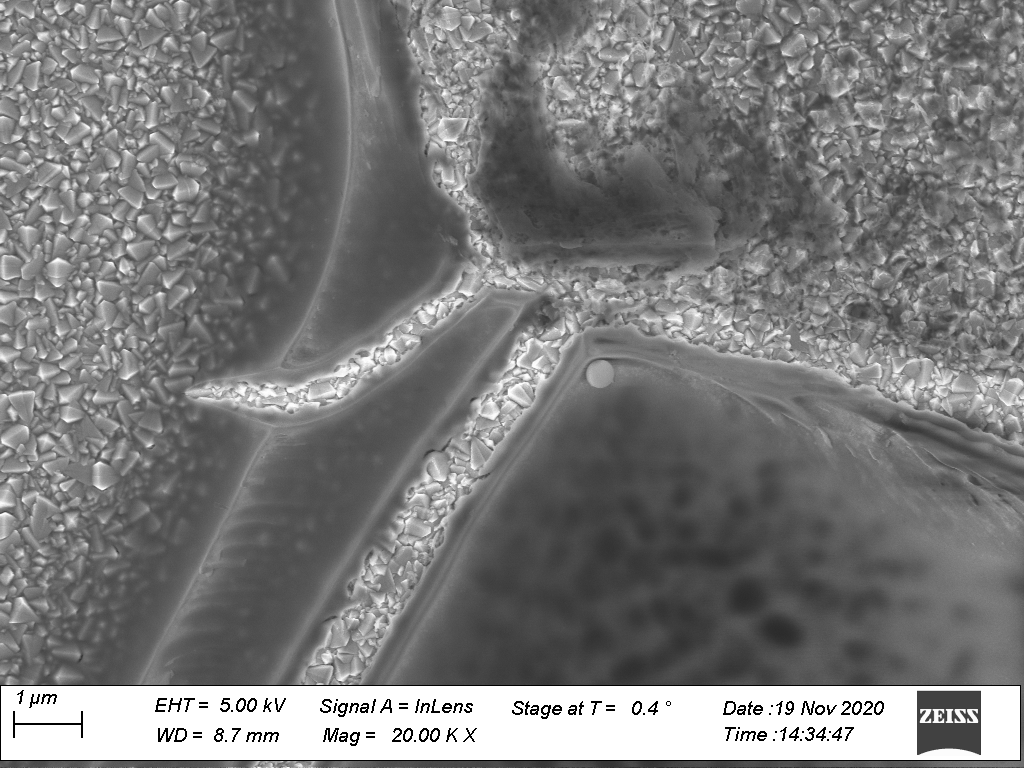
\includegraphics[width=\textwidth]{Pics/sem/071_fto_old_1x.png}
        \caption{sem1}
        \label{fig:sem1}
    \end{subfigure}
    \begin{subfigure}{.4\textwidth}
        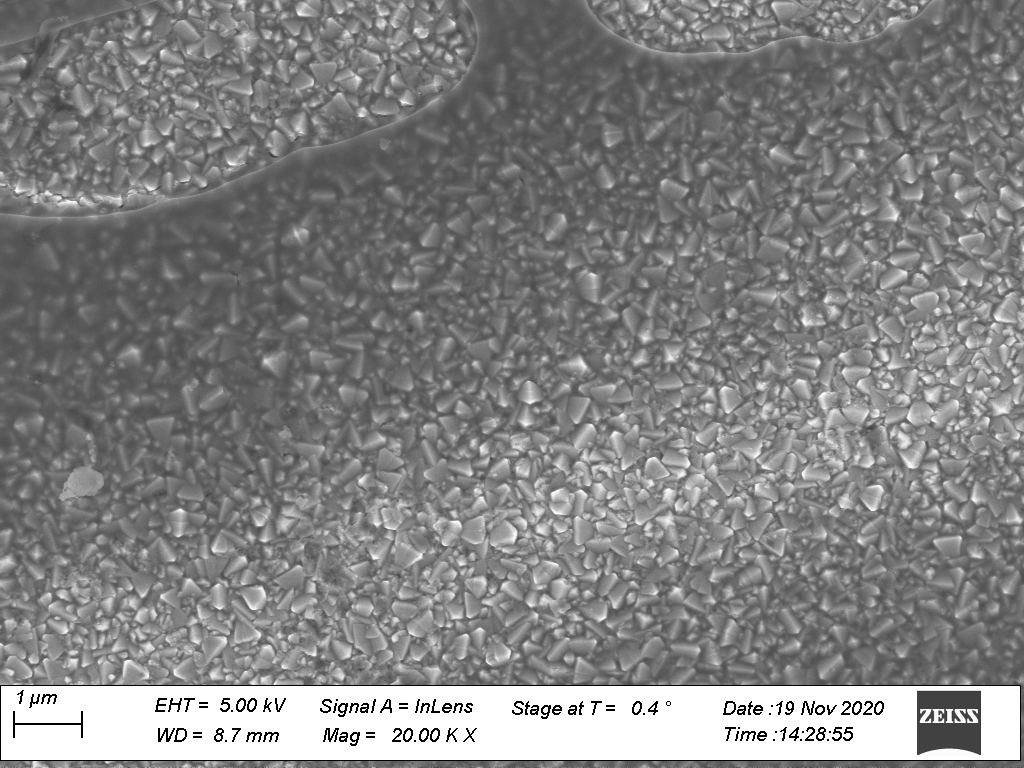
\includegraphics[width=\textwidth]{Pics/sem/071_fto_old_2x.png}
        \caption{sem2}
        \label{fig:sem2}
    \end{subfigure}
    \caption{sem}
    \label{fig:sem}
\end{figure}


%%%%%%%%%%%%%%%%%%%%%%%%%%%%%%%%%%%%%%%%%%%%%%%%%%%%%%%%%%%
%%%%%%%%%%%%%%%%%%%%%%%%%%%%%%%%%%%%%%%%%%%%%%%%%%%%%%%%%%%
\subsection{Material Scientific}
\subsubsection{First recipe} 
As already indicated in the experimental section the recipe adopted from \cite{Anwar2017} didn't produce any \td{good} results. 
The solution was milky/cloudy and didn't produce homogeneous films. 
Altering the composition, pH, surfactant etc. didn't improve the resulting layers. 
%- first recipe tried to improve to achieve more restisting layer. by pH value, surface tension and solution ratios (only 10\% change because it was assumed, that the recipe is good and should be improved, but the recipe should be altered thoroughly. two layers were also tried but didn't even pass the visual examination/test/inspection. A curst was produced. 

The sol-gel recipe optimized by \cite{Hu2016} for \ch{Al2O3} worked splendidly for our use even after (not so) minor changes.
%An substantial improvement could be achieved by
The stability of the solution could be increased a lot by replacing the stabilizing agent (\gls{acoh}) with \gls{ipo}.
The stability was inspected visually. 
As soon as the solution showed initial cloudiness, it was declared as unstable. 
The regular solution was stable for approximately \td{24h} sealed with Parafilm. 
%192 was first with IPOH
A solution with \gls{ipo} as stabilizing agent stayed stable for \td{72h}. 
As an increase of the \gls{zrpro} concentration decreased the \td{stable time}. 
%5F ca 100min
%4F ca 140min
%3F ca 420min (7h)
%extra AcOH stabilzed but needed so much that dilution too large...
%\td{IPO influence on "stability" p74: 600ul IPO makes clear, 4000 ul BuOH not clear with 
%same base solution (1ml of 4F), added extra 400ul to BuOH sol and after 5min clear. 
%of 1:5 is unacceptable Dilution }
%- 21.8 (1F) from 15.02. 13:30 bis 
%26.3 (1ml iPO to ca2ml of 5f) from 16.02. 16:30 bis 18.02.++
%18.02 4F in 80min milky
%      2F in ca 24h (stabilization AcOH)
%
%acceptable layer was produced by buthanolic solution, but very unstable (short lived) how long? p41 
\Gls{ipo} solution allowed to even reuse high concentrated solution, which would otherwise become cloudy under 60 minutes. 
Multiple question still need to be answered: 
What causes the cloudiness (as stability increased through sealing probably \ch{H2O} from the air or \ch{O2}) and what's the mechanism? 
How does \gls{ipo} increase the stability? 
Does it do so because it "fits" better with the solvent. 
As the original solvent was 2-methoxy-ethonanol instead of \ch{buoh}. 
It was even observed that the addition of \td{some drops of} \gls{ipo} to an acetic solution can clear the solution.
5F acetic solution milky over night 5:1 dilution with \gls{ipo} and clear after one minute of stirring and stayed clear over 5 nights.
% more details on pages 68ff
No effect on the solution or the resulting layer was noticed \td{from the initial stirring}
\todo{Following stirring times (in minutes) were tested and didn't have an influence on stability of the solution: 10-10-20, 10-10-45, 30-30-180.}
%The stirring time was untersucht, but not much difference so shortest was used because 
%short time can produces faster and the resulting solution is longer stable 
%(after finishing mixing)

%\td{instead of changing the stabilisation agent before optimisation, could change after pso, was vor und nachteile?}
after realizing the improved effectiveness of \gls{ipo} for experimentation, 
it was decided that EMMA will be executed with \gls{ipo} solution.
\begin{figure}
    \centering
    \begin{subfigure}{.3\textwidth}
        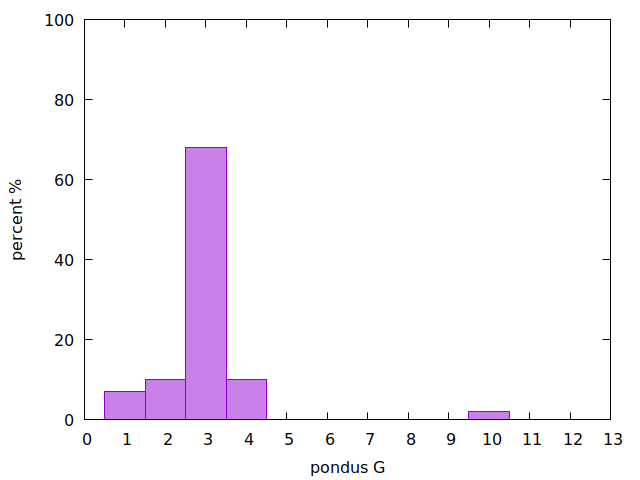
\includegraphics[width=\textwidth]{Pics/iv/iv-199-acoh.png}
        \caption{iv acoh} \label{fig:iv-acoh}
    \end{subfigure}
    \begin{subfigure}{.3\textwidth}
        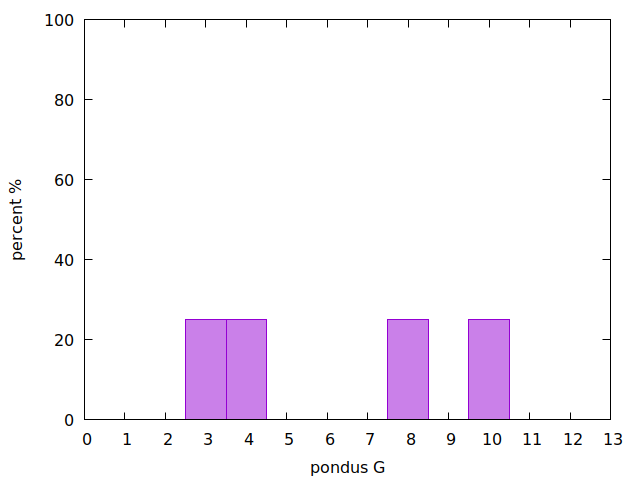
\includegraphics[width=\textwidth]{Pics/iv/iv-201-acoh-ipo.png}
        \caption{iv acoh ipo} \label{fig:iv-acoh-ipo}
    \end{subfigure}
    \begin{subfigure}{.3\textwidth}
        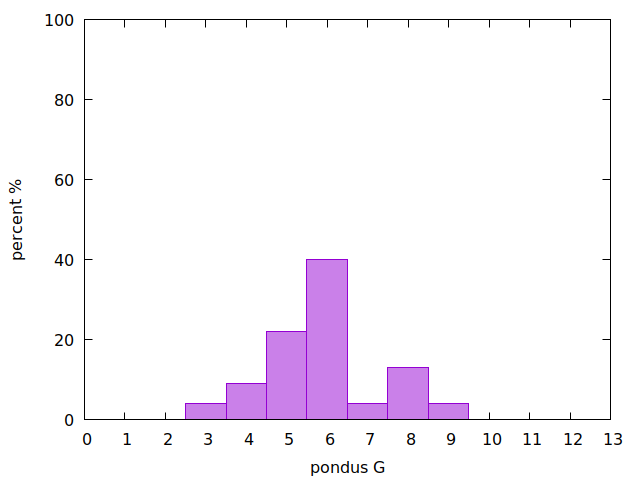
\includegraphics[width=\textwidth]{Pics/iv/iv-192-ipo.png}
        \caption{ipo} \label{fig:ipo}
    \end{subfigure}
    \caption{iv of 6x4F} \label{fig:iv}
\end{figure}

%%%%%%%%%%%%%%%%%%%%%%%%%%%%%%%%%%%%%%%%%%%%%%%%%%%%%%%%%%%
%%%%%%%%%%%%%%%%%%%%%%%%%%%%%%%%%%%%%%%%%%%%%%%%%%%%%%%%%%%
\subsection{V-I and preoptimization}
The doctor blading velocity (i.e. the velocity with which the blade moves and spreads the sol over the sample) 
was varied during preoptimization. 
The slower the \gls{db} velocity the more \td{homogeneously} the solution evaporated. 
If the \gls{db} was \td{too slow (lt 1 mm/s)} the surface tension pulled solvent over the sample without \td{leaving was zurk/forming a gel.}
\td{deposition because miniscus is pulling liquid off the substrate.}
Additionally the temperature while doctor blading affects the resulting layer together with the \gls{db} velocity. 

\td{Assumption: Ideally solution evaporate shortly after DB but not before}
due to the boiling point of \gls{buoh} at 117 C\cite{ncbi1butanol} the room temperature to 80 C were used as temperature during \gls{db}.
- p76, 146 (10x1F) good, 154 (3x4F) okay, 156 (3x3F) bad visualisation
\begin{figure}
    \centering
    \begin{subfigure}{.3\textwidth}
        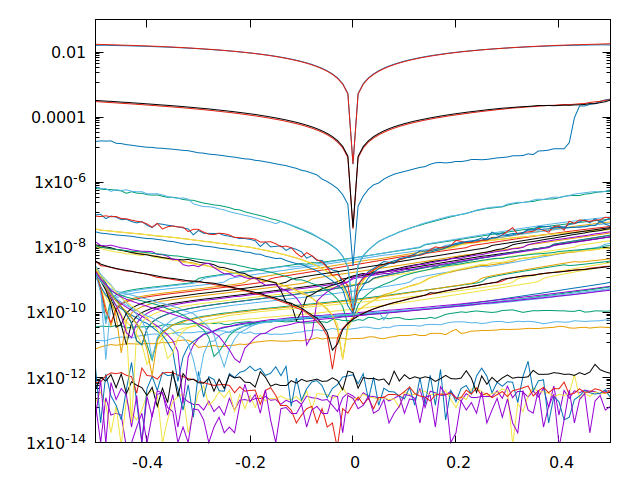
\includegraphics[width=\textwidth]{Pics/iv/log-146-good-10x1F.png}
        \caption{log} \label{fig:log1}
    \end{subfigure}
    \begin{subfigure}{.3\textwidth}
        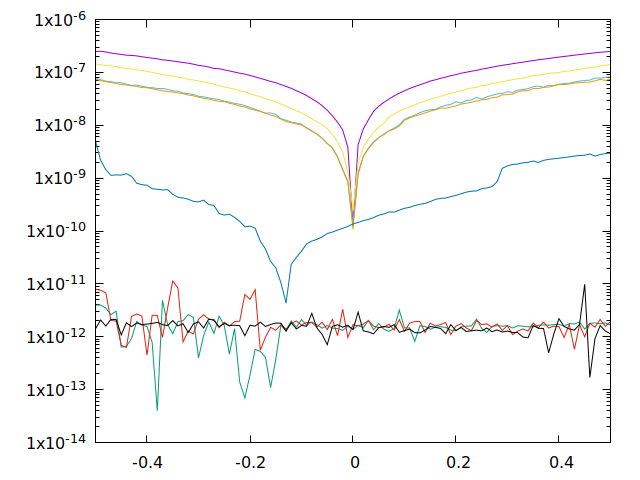
\includegraphics[width=\textwidth]{Pics/iv/log-154-okay-3x4F.png}
        \caption{log} \label{fig:log2}
    \end{subfigure}
    \begin{subfigure}{.3\textwidth}
        \includegraphics[width=\textwidth]{Pics/iv/log-156-bad-3x3F.png}
        \caption{log} \label{fig:log3}
    \end{subfigure}
    \begin{subfigure}{.3\textwidth}
        \includegraphics[width=\textwidth]{Pics/iv/stat-146-good-10x1F.png}
        \caption{stat} \label{fig:stat1}
    \end{subfigure}
    \begin{subfigure}{.3\textwidth}
        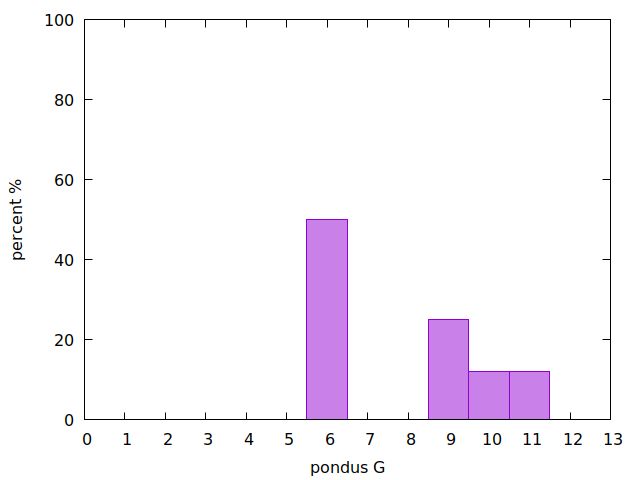
\includegraphics[width=\textwidth]{Pics/iv/stat-154-okay-3x4F.png}
        \caption{stat} \label{fig:stat2}
    \end{subfigure}
    \begin{subfigure}{.3\textwidth}
        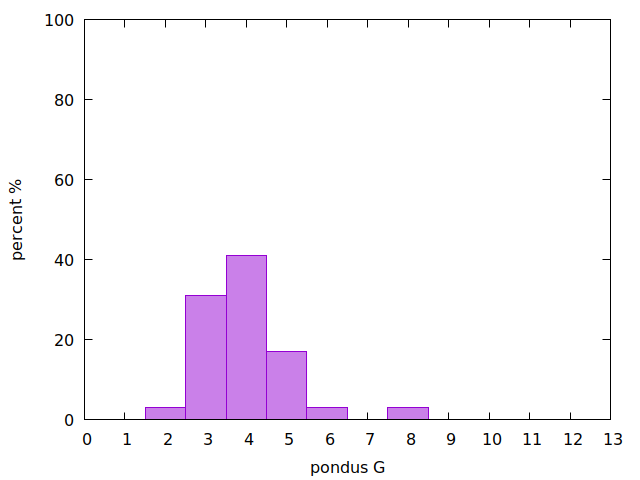
\includegraphics[width=\textwidth]{Pics/iv/stat-156-bad-3x3F.png}
        \caption{stat} \label{fig:stat3}
    \end{subfigure}
    \caption{maybe remove 146 and make 154 good AND set yrange [E-1:E-14]} \label{fig:sem}
\end{figure}


